%WI-FI(Arsitektur Komputer)
%Kelas: D4 TI 1B
%Alit Fajar Kurniawan(1174057)
%Berlian Nugraha Indra Maha Putra(1174058)
%Ichsan Hizman Hardy(1174034)
%Iqbal Hambali(1174060)
%Kevin Natanael Nainggolan(1174059)
%Virga Ukhu Ismada Yudha(1174065)
%Yusri Rizal(1154072)

\section {Wi-Fi (Wireless Fidelity)}
Wireless Fidelity merupakan suatu standart wireless networking atau tanpa kabel. teknologi spesifikasi ini emiliki standart yang 
ditetapkan oleh sebuah institusi internasional yang bernama IEEE  (Insitute of Electrical and Electronic Engineers). Di tahun 1997 
sebuah lembagaindependen bernama IEEE membuat standart WLAN pertama yang diberi kode 802.11. dapat bekerja pada frekuensi 2,4GHz 
dengan kecepatan transfer data 2Mbps.

Empat sejarah singkat perkembangan protokol Wireless fidelity:

1. pada bulan juli tahun 1999, IEEE merilis spesifikasi baru yang bernama 802.11b. dengan kecepatan transfer data maksimal11Mbps.

2. pada waktu yang hampir sama institute of electrical and electronic engineers menggunakan teknik berbeda dalam membuat spesifikasi 
802.11a. Frekuensi yang  digunakan /"5GHz", dan sampai 54Mbps dalam memindahkan dan menyalin data

3. pada tahun 2002. institute of electrical and electronic engineers membuat spesifikasi baru yang dapat menggabungkan kelebihan antara 
802.11b dengan 802.11a. Spesifikasi baru yang diberi kode 802.11g ini bekerja pada frekuensi 2,4GHz dengan kecepatan transfer data 
maksimal 54Mbps.

4. di tahun 2006 institute of electrical and electronic engineers mengembangkan teknologi terbarunya dengan menggabungkan teknologi 
802.11b dengan 802.11g menjadi 802.11n. teknologi ini dikenal dengan istilah MIMO (Multiple Input Multiple Output) teknologi wireless 
fidelity terbaru
 
\subsection {SEJARAH WI-FI}
HI-FI merupakan asal mula sebelum adanya WI-FI yang terdiri dari jenis output yang dihasilkan oleh kualitas sound system. Teknologi Wireless Fidelity berspesifikasi standart Institute of Electrical and Electronic Engineers atau yang disingkat dengan IEEE 802.. termasuk 802.11a, 802.11b, dan 802.11g. Wireless Fidelity adalah hanya istilah produk teknologi yang dipromosikan oleh WIFI Alliance.
Sejarah Wireless Fidelity itu sendiri dimulai ketika tahun 1985 dari hasil kerja keras insinyur Amerika dengan pengguna Teknologi penyebaran spektrum radio yang digunakan dalam Wi-Fi. Wireless LAN atau Wi-Fi dibuat dan tersedia untuk umum di Amerika Serikat di tahun 1985, tidak ada lisensi dari komisi komunikasi federal (FCC). Kemudian Michael Marcus mengusulkan untuk menggunakan wireless LAN dan teknologi radio untuk publik.

Wi-Fi adalah sebuah teknologi yang memanfaatkan peralatan teknologi untuk bertukar data menggunakan gelombang radio melalui jaringan komputer. Vic Hayes adalah penemu Wi-Fi yang kini dijuluki sebagai “ Father of Wi-Fi “. WI-Fi merupakan sekumpulan standar yang digunakan untuk Jaringan Lokal Nirkabel yang memiliki spesifikasi IEEE 802.11. Pengertian dari IEEE tersebut adalah sebuah organisasi internasional yang mempublikasikan beberapa persoalan kunci dari dunia networking komputer. Ada awalnya Wi-Fi hanya digunakan pada jaringan Lokal (LAN),seiring berjalannya waktu Wi-Fi dimanfaatkan masyarakat untuk mengakses internet. Penerapan Wi-Fi  ditujukan sebagai alternatif dari jaringan Lokal komputer LAN,dimana penggunaan kabel sudah tidak lagi effisien. Wi-Fi memiliki mobilitas yang tinggi,sehingga untuk mengakses WI-Fi ini tidak diperlukannya penyambung kabel untuk menghubungkan ke server.
Pada dasarnya,Wi-Fi terdiri dari sumber yang dihubungkan dengan access point melalui kabel backbone. Selanjutnya dipancarkan melalui gelombang elektromagnetik seperti pada LAN kabel biasa yang kemudian diterima oleh client (Contohnya PC desktop) melalui wireless adapter yang mendukung jaringan Wi-Fi berdasarkan standarisasi IEEE 802.11. Tetapi access point ini memiliki area yang sangat terbatas,500 feet (152.4 M) dalam ruangan tertutup dan 1000 feet (304.8 M) dalam ruangan terbuka.
Wi-Fi akan mengalami proses handoffs agar wireless client dapat melanjutkan komunikasi dengan server yang berbeda. Wireless client akan terus memonitor sinyal yang diterima oleh access point,jika kuat sinyal kurang dari nilai sensitivitas penerimaan (threshold) maka wireless akan melakukan handoffs yang selanjutnya akan mencari sinyal terdekat. Proses identifikasi dari wireless client untuk menemukan sinyal access point terkuat hanya dibatasi dalam waktu 60 second. Backbone search time adalah proses pencarian AP dan EP untuk dijadikan BSS. Untuk dapat berkomunikasi yang lama antara wireless client dengan access point harus memiliki level daya yang diterima di atas -77 dBm,jika kurang dari -77 dBm maka wireless client akan melakukan proses handoffs dengan beralih pada daya yang lebih tinggi dari access point sebelumnya.
Dibalik kelebihannya Wi-Fi yang sudah memiliki kebutuhan  akses internet yang lebih baik dibandingkan dengan akses internet yang menggunakan kabel,tetapi Wi-Fi masih memiliki beberapa kekurangan sekarang ini,diantaranya ada :
	Area coverage-nya yang sangat sempit,hanya dalam hitungan meter
	Hanya mencukupi akses internet dalam suatu daerah atau dalam ruangan saja
	Keamanan yang belum terjamin
	Membutuhkan banyak BTS untuk menjangkau seluruh area yang luas
	LoS (Line of Sight)


\subsection {Cara Kerja Wi-Fi}
 Mode Akses Koneksi Wi-fi ada 2 yaitu :
1. AD-HOC
sisrem Ad-hoc atau pun biasa disebut denan sistem peer to peer yang berarti yaitu membuat jaringan menjadi lebih luas atau bisa juga 
disebut dengan hotspot, dalam arti satu computer dihubungkan ke 1 computer dengan mengetahui SSID dari setiap komputer. Bila digambarkan 
mungkin lebih mudah membayangkan sistem direct connection dari 1 computer ke 1 computer lainnya dengan mengunakan Twist pair cable tanpa 
memerlukan prangkat HUB. Jadi terdapat 2 computer dengan perangkat WIFI yang dapat langsung berhubungan tanpa alat yang disebut access 
point mode. Pada sistem Adhoc ini tidak lagi mengenal system central atau yang biasanya difungsikan pada Access Point. Sistem Adhoc hanya 
memerlukan 1 buah computer yang memiliki nama SSID atau sering disebut juga network pada sebuah card/computer. Dapat juga mengunakan MAC 
address dengan sistem BSSID, untuk mengenal sebuah nama computer secara langsung. Mac Address umumnya sudah diberikan tanda atau nomor 
khusus tersendiri dari masing masing card atau perangkat network termasuk network wireless. Sistem Adhoc menguntungkan untuk pemakaian
sementara misalnya hubungan network antara 2 komputer walaupun disekitarnya terdapat sebuah alat Access Point yang sedang bekerja.

2. INFRASTRUKTUR
Sistem kedua yang paling umum adalah Infra Struktur. Sistem Infra Struktur membutuhkan sebuah perangkat yang khusus, atau dapat digunakan 
sebagai Access point melalui software apabila menggunakan jenis Wireless Network dengan perangkat PCI card. Mirip Hub Network yang 
menyatukan sebuah sambungan tetapi di dalam perangkat Access Point menandakan sebuah central network dengan memberikan sinyal 
radio untuk diterima oleh komputer lain. Untuk mengambarkan koneksi pada Infra Struktur dengan Access poin minimal 
sebuah jaringan wireless network memiliki satu titik pada sebuah tempat dimana komputer lain yang mencari dan menerima sinyal untuk masuknya 
kedalam network agar saling berhubungan. Sistem Access Point (AP) ini  paling banyak digunakan karena setiap komputer yang ingin 
terhubung kedalam network dapat mendengar transmisi dari Access Point tersebut. Access Point inilah yang memberikan
tanda apakah disuatu tempat memiliki jaringan WIFI atau tidak dan secara terus menerus mentransmisikan namanya – Service Set Identifier dan dapat diterima oleh komputer lain untuk dikenal. Bedanya Access point dengan HUB network cable,yaitu HUB mengunakan cable tetapi 
tidak memiliki nama (SSID). Sedangkan Access point tidak mengunakan kabel network tetapi harus memiliki sebuah nama yaitu nama untuk SSID.
Contoh Wi-fi Hardware yang digunakan di masyarakat : Wi-fi dalam bentuk PCI Wi-fi dalam bentuk USB


\subsection {Perbedaan antara WI-FI dengan WIMAX}

Pada awalnya WI-FI dan WIMAX tidak memiliki banyak perbedaan, hanya perbedaan antara jarak jangkauan luas jaringan nya.
jika WI-FI hanya mampu menyalurkan sinyalnya hanya sampai beberapa meter saja dan semakin jauh jangkauan si pemakai WI-FI maka
semakin kecil pula sinyal yang diterimanya. Berbeda dengan WIMAX yang memiliki cakupan coverage area lebih luas atau jangkauan 
sinyalnya lebih luas.

\subsection{Teknik pelokalan WiFi}

Teknik pelokalan WiFi masuk dalam sejumlah kategori besar. Beberapa teknik estimasi lokasi mencoba Model propagasi sinyal secara 
langsung melalui ruang [Bahl dan Padmanabhan, 2000], dengan asumsi lokasi akses diketahui titik dan model atenuasi sinyal eksponensial. 
Namun, bahkan saat mempertimbangkan lokasi dan material dinding dan furnitur di dalam bangunan, keakuratan perambatan sinyal Modelnya 
sangat terbatas. Teknik lain mencoba model kemungkinan membaca berdasarkan lokasi spesifik [Haeberlen et al., 2004; Letchner et al., 
2005], mewakili kekuatan sinyal di lokasi yang diminati dengan distribusi probabilitas yang dipelajari dari data pelatihan Sedangkan 
lebih akurat dibanding propagasi sinyal model, metode ini secara inheren diskrit dan memiliki hanya kemampuan terbatas untuk interpolasi 
antar lokasi. Untuk mengatasi keterbatasan tersebut, Schwaighofer dan rekannya [2003] menunjukkan bagaimana menerapkan proses Gaussian 
ke lokalisasi kekuatan sinyal, menghasilkan model yang disediakan interpolasi melalui lokasi kontinu dengan pemodelan langsung
ketidakpastian dari data pelatihan [Ferris dkk, 2006] diperpanjang Teknik ini untuk lokalisasi WiFi dengan menggabungkan Model kekuatan 
sinyal GP dengan graph-based tracking, memungkinkan untuk lokalisasi yang akurat dalam skala skala besar.

\subsection{Jenis jenis Wireless}
1. Berbasis Ad-Hoc
Pada jaringan ini, komunikasi antara satu perangkat ke perangkat lain di lakukan secara
spontan atau langsung tanpa melalui konfigurasi tertentu selama Acces point masih dapat
diterima dengan baik oleh perangkat perangkat lain dalam jaringan ini.

\begin{figure}[ht]
\centerline{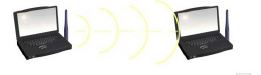
\includegraphics[width=0.1\textwidth]{figures/wlan1.jpg}}
\caption{WLAN Ad-Hoc}
\label{wlan}
\end {figure}

2. Berbasis Infrastruktur
Pada jaringan ini, satu atau lebih Acces Point menghubungkan jaringan WLAN melalui
jaringan berbasis kabel. Jadi pada jaringan ini, untuk melayani perangkat didalam
jaringan ini maka Acces Point memerlukan koneksi ke jaringan berbasis kabel terlebih
dahulu.

\begin{figure}[ht]
\centerline{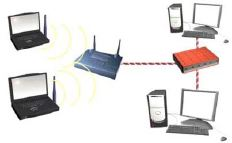
\includegraphics[width=0.1\textwidth]{figures/wlan-infrastruktur3.jpg}}
\caption{WLAN yang Berbasis Infrastruktur}
\label{wlan-infrastruktur}
\end {figure}

Karena banyak nya jenis jenis WLAN yang ada di pasaran, maka standar IEE 802.11
menetapkan antarmuka yang klien WLAN dengan Acces Point nya. Untuk membedakan
antara jariangan WLAN satu dengan jaringan WLAN lain nya, maka 802.11
menggunakan Service Set Identifier ( SSID ). Dengan penanda ini maka dapat dibedakan
jaringan WLAN satu dengan jaringan WLAN lain nya, sebab jaringan WLAN satu
dengan jaringan WLAN yang lain nya pasti memiliki nomor penanda SSID yang berbeda
pula. Acces Point menggunakan SSID untuk menentukkan lalu lintas paket data mana
yang di peruntukkan untuk Acces Point tersebut.
Standar 802.11 juga menentukkan frekuensi yang dapat di gunakan oleh jaringan WLAN.
Misal nya untuk industrial, scientific dan medical ( ISM) beroperasi pada freukensi radio
2,4GHz. 802.11 juga menentukkan tiga jenis tranmisi pada lapisan fisik untuk model
Open System Interconnection ( OSI ), yaitu direct-sequence spread spectrum ( DSSS ),
frecuency-hopping spread spectrum ( FHSS ), dan infrared. Selain pembagian frekuensi
di atas, standar 802.11 juga membagi frame nya menjadi tiga kategori, yaitu control, date
dan management.
Standar 802.11 membolehkan device ( perangkat ) mengikuti standar 802.11 untuk
berkomunikasi satu sama lain nya dengan kecepatan 1Mbps dan 2Mbps dalam jangkauan
kira kira 100 meter. Jenis lain dari standar 802.11 nanti di kembangkan untuk
menyediakan kecepatan transfer data yang lebih cepat dengan tingkat fungsionalitas yang
lebih baik dari yang ada saat ini. Saat ini terdapat beberapa jenis variant dari standar
802.11, yaitu 802.11a, 802.11b, dan 802.11g.
Di bandingkan dengan standar 802.11a, ternyata standar 802.11g memiliki kelebihan
kompatibilitas dengan jaringan standar 802.11b. Namun, masalah yang sering muncul
adalah perangkat perangkat standar 802.11g yang mencoba berpindah ke jaringan standar
802.11b atau sebalik nya adalah masalah interfensi yang di akibatkan jaringan frekuensi
2,4GHz.

\subsection {Perkembangan}
Perkembangan teknologi perangkat komunikasi data melalui jaringan nirkabel atau Wireless LAN (WLAN) terus meningkat sejalan dengan 
penggunaan akses internet yang makin hari semakin banyak. Teknologi Wireless LAN yang direkomendasikan melalui standar IEEE 802.11 
ada tiga, yaitu : Standar IEEE 802.11, Standar IEEE 802.11a, 
Standar IEEE 802.11b dan Standar IEEE 802.11g. Wireless fidelity atau yang sering 
kita kenal sebagai Wi-Fi merupakan teknologi WLAN dengan standar IEEE 802.11b yang beroperasi di frekuensi 2,4 GHz-2,5 GHz. Antena Access 
Point dalam stuktur jaringan WLAN mempunyai fungsi sebagai media yang mendistribusikan sinyal ke beberapa perangkat bergerak atau mobile 
station. Untuk meningkatkan kemampuan daya transmisi sinyal dan daya jangkauan pancaran gelombang elektromagnetik lebih jauh.Untuk 
menunjang kemampuan tersebut dalam riset ini di rancang antena dasar bersifat susun array. Antena pada titik akses memiliki sifat 
directional. Sehingga antena dapat dirancang dengan model susun agar memperoleh gain yang lebih tinggi. Antena susun dua patch 
terdistribusi melalui rangkaian transformer seperempat, gelombang menggunkan model power divider T-Juntcion atau cabang tiga. Rangkaian transformer 
dirancang melalui saluran transmisi mikrostrip dengan struktur terdiri dari dua saluran keluaran dan satu saluran masuk yang memiliki 
nilai impedansi sama. Penempatan antar patch peradiasi secara linier satu sumbu koordinat dengan pengaturan jarak resonansi di atas 
seperempat gelombang pada titik pusat patch peradiasi. Material substrat PCB yang digunakan jenis duroid 5880 dengan ketebalan 1,57 mm dan
konstanta dielektrik. Untuk rancang bangun antena digunakan metode simulasi menggunakan perangkat lunak microwave office. Hasil rancang bangun antena susun dua patch diharapkan tercapai target parameter gain diatas 5 dB.
 
 \cite {yustiyan2006analisa}
 \cite {arief2007teknologi}
 \cite {darsono2012rancang}
 \cite {yudianto2007jaringan}